% Created 2016-08-17 Wed 14:38
\documentclass[tikz]{standalone}

\usepackage[utf8]{inputenc}
\usepackage[T1]{fontenc}

\usepackage{circledsteps}

\RequirePackage{xcolor}

%% HPI color definitions according to the design manual
% These do not exactly match the RGB values used in the Powerpoint slide master due to unknown reasons
\definecolor{hpiyellow}{RGB}{246,168,0}
\definecolor{hpiorange}{RGB}{221,97,8}
\definecolor{hpired}{RGB}{177,6,58}
\definecolor{hpigray}{RGB}{90,96,101}
\definecolor{hpiblue}{RGB}{0,122,158}


\renewcommand{\sfdefault}{neosans}
% Different font weights for neosans
\newcommand{\textl}[1]{{\fontseries{l}\selectfont #1}} % light
\newcommand{\textm}[1]{{\fontseries{m}\selectfont #1}} % medium, same as default weight
\newcommand{\textsb}[1]{{\fontseries{sb}\selectfont #1}} % semibold
\newcommand{\textmb}[1]{{\fontseries{mb}\selectfont #1}} % bold, same as \textbf
\newcommand{\texteb}[1]{{\fontseries{eb}\selectfont #1}} % extra bold
\newcommand{\textub}[1]{{\fontseries{ub}\selectfont #1}} % ultra bold

\tikzset{every picture/.style={/utils/exec={\sffamily}}}
\tikzset{flipflop RSflanke/.style={
  flipflop,
  flipflop def={t1=S, t2=C, c2=1, t3=R, t6=Q, t4={\ctikztextnot{Q}}}
}}


\tikzset{
  mechanicalSwitch/.pic={
    \coordinate (-inUp) at (135:2); 
    \coordinate (-inDown) at (235:2);
    \coordinate (-out) at (2,0);
    \coordinate (-center) at (0,0);
    
    \draw (0,0) circle [radius = 2cm];
    \draw [fill=gray!20] (0,0) circle [radius = 0.2cm];

    \draw (0, 0) -- (2, 0);
    \draw (135:.8) -- (135:2); 
    \draw (225:.8) -- (225:2); 

    \draw [fill=gray!20] (2, 0) circle [radius=0.05cm]; 
    \draw [fill=gray!20] (135:2) circle [radius=0.05cm]; 
    \draw [fill=gray!20] (225:2) circle [radius=0.05cm]; 

    
    \draw [thick] (0,0) -- (175:1.5); 

    \draw [dashed, <->, domain=135:225] plot ({cos(\x)}, {sin(\x)}); 
  },
  mechanicalSwitchClosed/.pic={
    \coordinate (-inUp) at (135:2); 
    \coordinate (-inDown) at (255:2);
    \coordinate (-out) at (2,0);
    \coordinate (-center) at (0,0);
    \draw (0,0) circle [radius = 2cm];
    \draw [fill=gray!20] (0,0) circle [radius = 0.2cm];

    \draw (0, 0) -- (2, 0);
    \draw (135:.8) -- (135:2); 
    \draw (225:.8) -- (225:2); 

    \draw [fill=gray!20] (2, 0) circle [radius=0.05cm]; 
    \draw [fill=gray!20] (135:2) circle [radius=0.05cm]; 
    \draw [fill=gray!20] (225:2) circle [radius=0.05cm]; 

    
    \draw [thick] (0,0) -- (135:2); 

    \draw [dashed, <->, domain=135:225] plot ({cos(\x)}, {sin(\x)}); 
  }
}


\usetikzlibrary{calc}
\usetikzlibrary{positioning}


\usetikzlibrary{calc,decorations.pathreplacing, chains,ext.positioning-plus}

\usepackage{pgfplots}

\begin{document}

\begin{tikzpicture}
  \label{page:phy:channel_bandwidth}
  \draw [->] (0,0) -- (0,5) node [left] {Attenuation}; 
  \draw [->] (0,0) -- (10,0) node [below] {Frequency};

  \draw (0.1,1) -- (-0.1,1)  node [left] {1}; 
  \draw (0.1, 2) -- (-0.1, 2)  node [left] {2}; 

  \draw [dashed] (0,2)  -- (10,2);
  \draw [dotted] (3,0) -- (3,2) (7,0) -- (7,2); 
  
  \draw (3, 0.1) -- (3, -0.1) node [below] {$f_1$}; 
  \draw (7, 0.1) -- (7, -0.1) node [below] {$f_2$};

  \draw (1, 5)  -- (3, 2) -- (4, 1.3) -- (5, 1.2) -- (6, 1.4)--  (7, 2) -- (8, 2.7) -- (9, 5) ;

  \draw [decorate, decoration={brace,mirror,raise=3pt}] (3,-1)  to node[below=0.5cm, align=center] (ll) {Channel bandwidth} (7, -1); 
\end{tikzpicture}

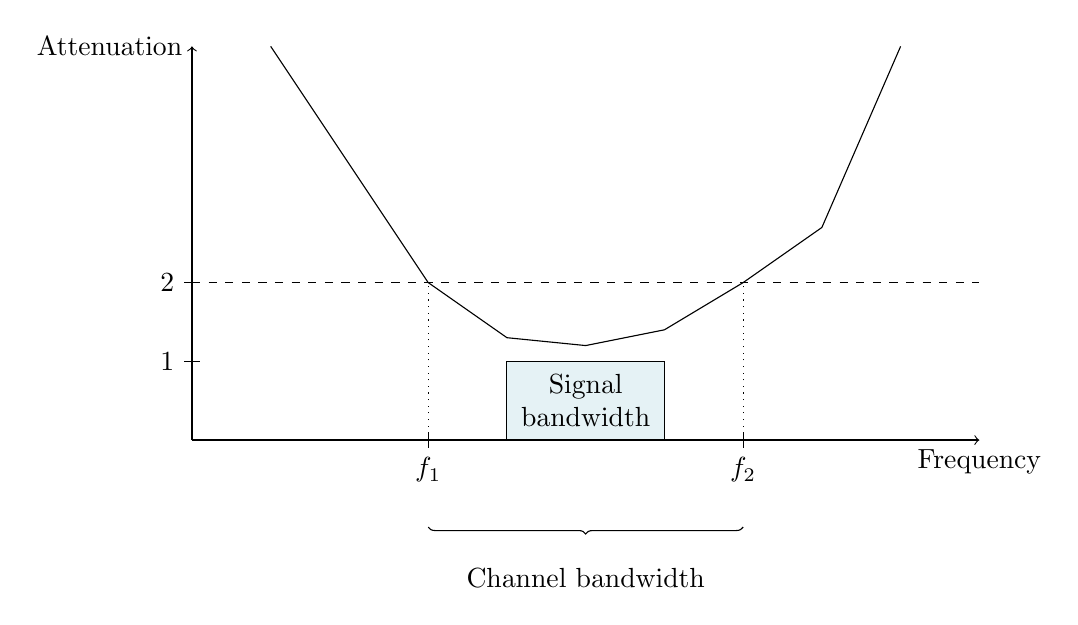
\begin{tikzpicture}
  \label{page:phy:channel_bandwidth:small_signalbw}
  \draw [->] (0,0) -- (0,5) node [left] {Attenuation}; 
  \draw [->] (0,0) -- (10,0) node [below] {Frequency};

  \draw (0.1,1) -- (-0.1,1)  node [left] {1}; 
  \draw (0.1, 2) -- (-0.1, 2)  node [left] {2}; 

  \draw [dashed] (0,2)  -- (10,2);
  \draw [dotted] (3,0) -- (3,2) (7,0) -- (7,2); 
  
  \draw (3, 0.1) -- (3, -0.1) node [below] {$f_1$}; 
  \draw (7, 0.1) -- (7, -0.1) node [below] {$f_2$};

  \draw (1, 5)  -- (3, 2) -- (4, 1.3) -- (5, 1.2) -- (6, 1.4)--  (7, 2) -- (8, 2.7) -- (9, 5) ;

  \draw [decorate, decoration={brace,mirror,raise=3pt}] (3,-1)  to node[below=0.5cm, align=center] (ll) {Channel bandwidth} (7, -1); 


  \draw [fill=hpiblue!10, draw] (4, 0) rectangle node[align=center] {Signal\\ bandwidth} (6, 1); 
  
\end{tikzpicture}

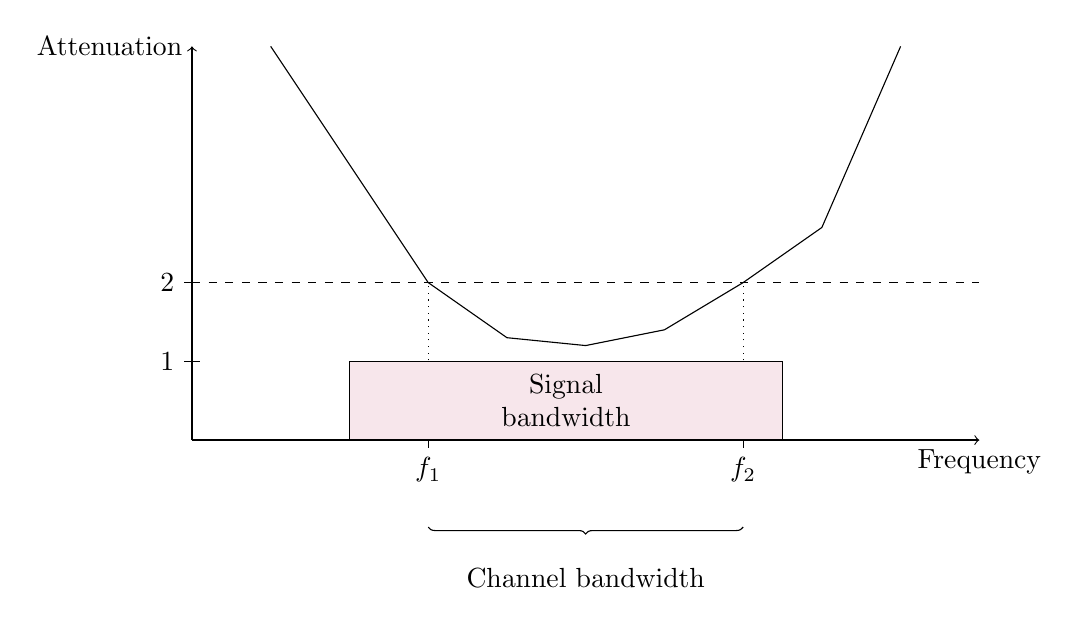
\begin{tikzpicture}
  \label{page:phy:channel_bandwidth:large_signalbw}
  \draw [->] (0,0) -- (0,5) node [left] {Attenuation}; 
  \draw [->] (0,0) -- (10,0) node [below] {Frequency};

  \draw (0.1,1) -- (-0.1,1)  node [left] {1}; 
  \draw (0.1, 2) -- (-0.1, 2)  node [left] {2}; 

  \draw [dashed] (0,2)  -- (10,2);
  \draw [dotted] (3,0) -- (3,2) (7,0) -- (7,2); 
  
  \draw (3, 0.1) -- (3, -0.1) node [below] {$f_1$}; 
  \draw (7, 0.1) -- (7, -0.1) node [below] {$f_2$};

  \draw (1, 5)  -- (3, 2) -- (4, 1.3) -- (5, 1.2) -- (6, 1.4)--  (7, 2) -- (8, 2.7) -- (9, 5) ;

  \draw [decorate, decoration={brace,mirror,raise=3pt}] (3,-1)  to node[below=0.5cm, align=center] (ll) {Channel bandwidth} (7, -1); 


  \draw [fill=hpired!10, draw] (2, 0) rectangle node[align=center] {Signal\\ bandwidth} (7.5, 1); 
  
\end{tikzpicture}


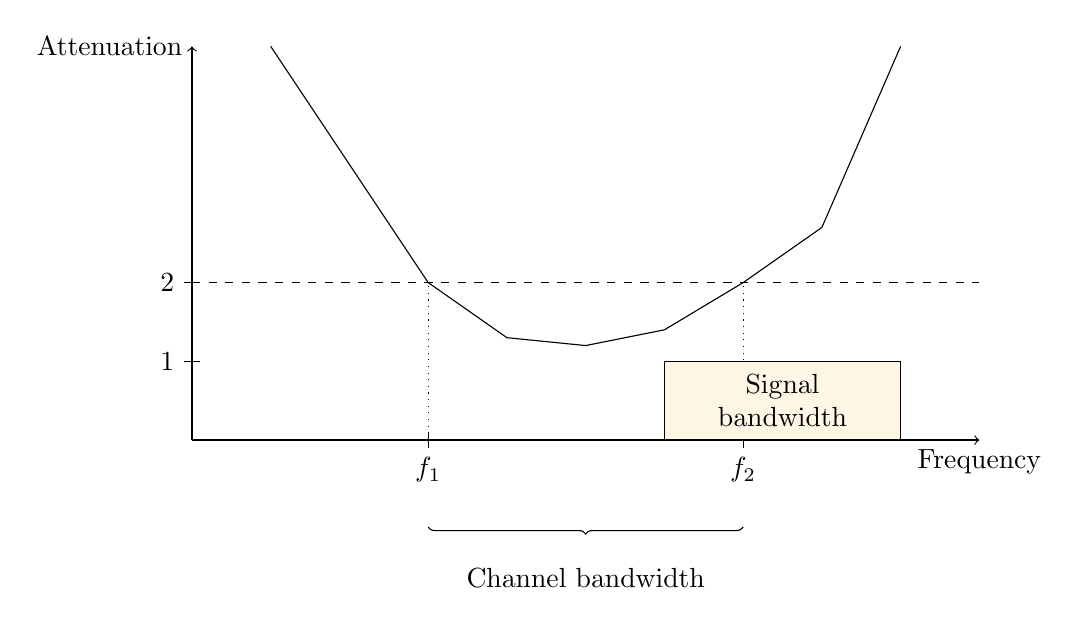
\begin{tikzpicture}
  \label{page:phy:channel_bandwidth:outside_signalbw}
  \draw [->] (0,0) -- (0,5) node [left] {Attenuation}; 
  \draw [->] (0,0) -- (10,0) node [below] {Frequency};

  \draw (0.1,1) -- (-0.1,1)  node [left] {1}; 
  \draw (0.1, 2) -- (-0.1, 2)  node [left] {2}; 

  \draw [dashed] (0,2)  -- (10,2);
  \draw [dotted] (3,0) -- (3,2) (7,0) -- (7,2); 
  
  \draw (3, 0.1) -- (3, -0.1) node [below] {$f_1$}; 
  \draw (7, 0.1) -- (7, -0.1) node [below] {$f_2$};

  \draw (1, 5)  -- (3, 2) -- (4, 1.3) -- (5, 1.2) -- (6, 1.4)--  (7, 2) -- (8, 2.7) -- (9, 5) ;

  \draw [decorate, decoration={brace,mirror,raise=3pt}] (3,-1)  to node[below=0.5cm, align=center] (ll) {Channel bandwidth} (7, -1); 


  \draw [fill=hpiyellow!10, draw] (6, 0) rectangle node[align=center] {Signal\\ bandwidth} (9, 1); 
  
\end{tikzpicture}

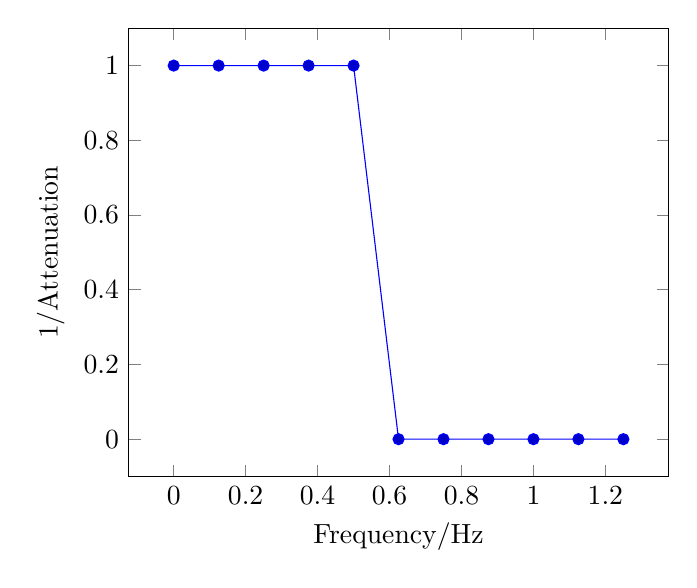
\begin{tikzpicture}
  \label{page:phy:lowpass:simplistic_attenuation}

  % compare in fourier.py: 
% def lowpass (t):
%    return c + sum (1./(i*i) * a(t, i) for i in range(1, 11))  + sum (1./(i*i) * b(t, i) for i in range(1, 11)) 
%    attenaution over frequencies:
%    f0=0, alpha 0 =1
%    f1 = 1/8 Hz, alpha = 1
  % f2 = 2 * 1/8 Hz, alpha = (1/2*2)^2 
  \begin{axis}
    [xlabel=Frequency/Hz, ylabel=1/Attenuation]
    \addplot coordinates {(0, 1) (0.125, 1)
      (2*0.125, 1)
      (3*0.125, 1)
      (4*0.125, 1)
      (5*0.125, 0)
      (6*0.125, 0)
      (7*0.125, 0)
      (8*0.125, 0)
      (9*0.125, 0)
      (10*0.125, 0)
    };
  \end{axis}
\end{tikzpicture}


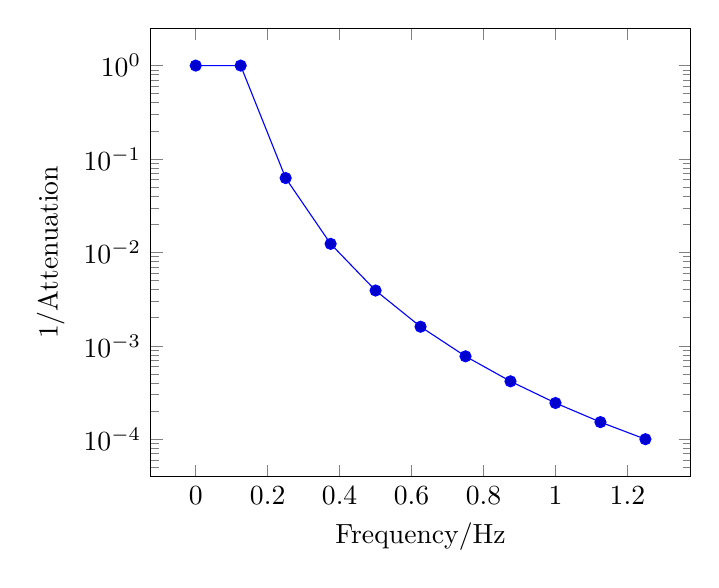
\begin{tikzpicture}
  \label{page:phy:lowpass:attenuation}

  % compare in fourier.py: 
% def lowpass (t):
%    return c + sum (1./(i*i) * a(t, i) for i in range(1, 11))  + sum (1./(i*i) * b(t, i) for i in range(1, 11)) 
%    attenaution over frequencies:
%    f0=0, alpha 0 =1
%    f1 = 1/8 Hz, alpha = 1
  % f2 = 2 * 1/8 Hz, alpha = (1/2*2)^2 
  \begin{semilogyaxis}
    [xlabel=Frequency/Hz, ylabel=1/Attenuation]
    \addplot coordinates {(0, 1) (0.125, 1) (2*0.125, 1/2*1/2*1/2*1/2)
      (3*0.125, 1/3*1/3*1/3*1/3)
      (4*0.125, 1/4*1/4*1/4*1/4)
      (5*0.125, 1/5*1/5*1/5*1/5)
      (6*0.125, 1/6*1/6*1/6*1/6)
      (7*0.125, 1/7*1/7*1/7*1/7)
      (8*0.125, 1/8*1/8*1/8*1/8)
      (9*0.125, 1/9*1/9*1/9*1/9)
      (10*0.125, 1/10*1/10*1/10*1/10)
    };
  \end{semilogyaxis}
\end{tikzpicture}

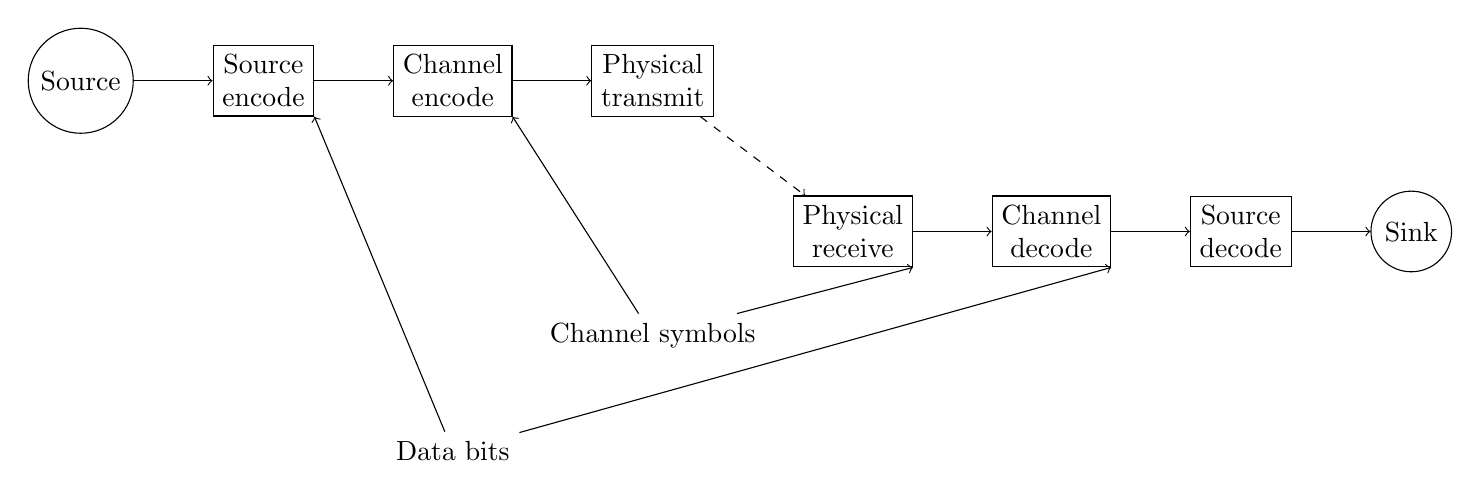
\begin{tikzpicture}[start chain=1, start chain=2, every join/.style={->}]
  \label{page:phy:structure:baseband}
  
  \begin{scope}[every node/.style={on chain=1, draw, align=center, join}]
    \node [circle] (source) {Source};
    \node (sencode) {Source\\encode};
    \node (chencode) {Channel\\encode};
    \node (tx) {Physical \\transmit};
  \end{scope}

  \begin{scope}[every node/.style={on chain=2, draw, align=center, join}]
    \node [below right=of tx] (rx) {Physical\\receive};
    \node (chdecode) {Channel\\decode};
    \node (sdecode) {Source\\decode};
    \node [circle] (sink) {Sink};
  \end{scope}

  \draw [->, dashed] (tx) -- (rx);

  \node [below=4 of chencode] (bits) {Data bits};
  \node [below=2.5 of tx] (symbols) {Channel symbols};

  \draw [->] (bits) edge (sencode.south east) edge (chdecode.south east); 
  \draw [->] (symbols) edge (chencode.south east) edge (rx.south east); 
\end{tikzpicture}

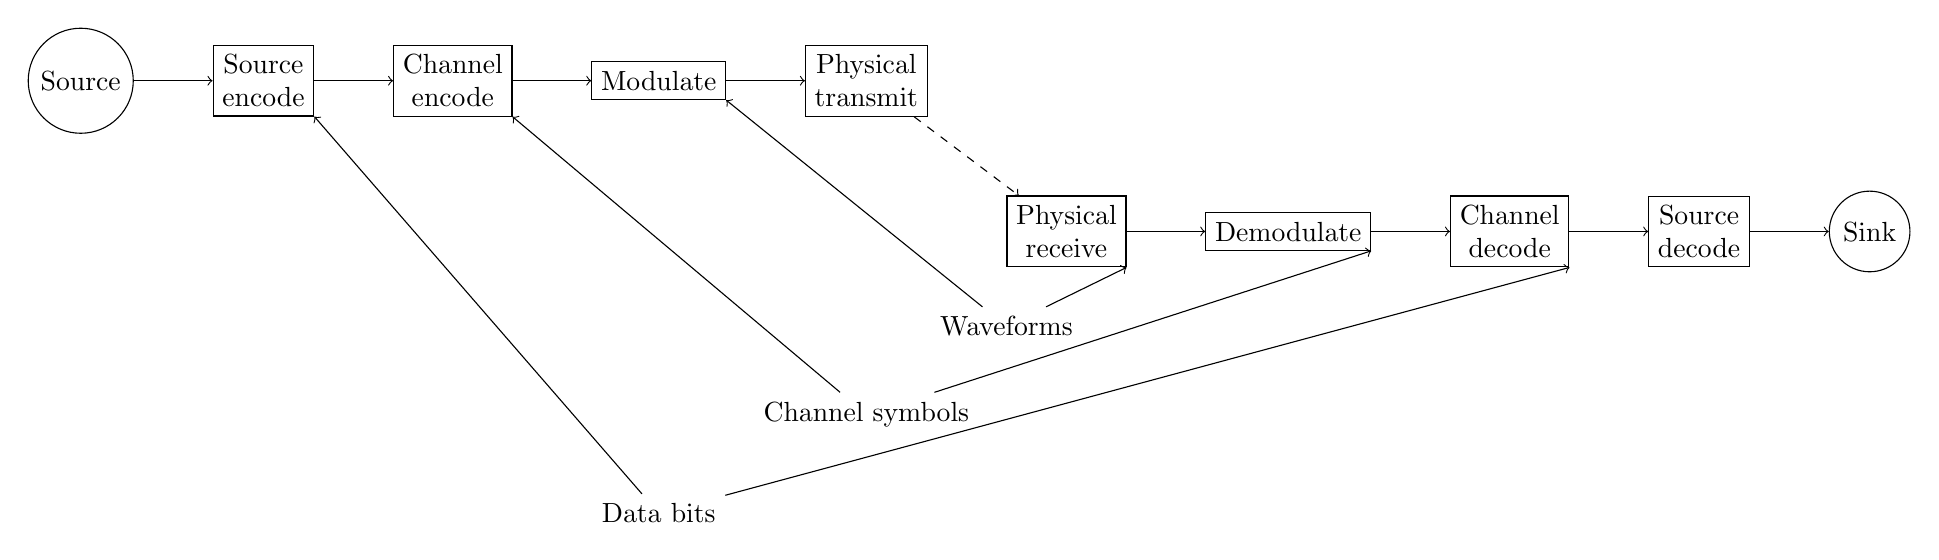
\begin{tikzpicture}[start chain=1, start chain=2, every join/.style={->}]
  \label{page:phy:structure:broadband}
  
  \begin{scope}[every node/.style={on chain=1, draw, align=center, join}]
    \node [circle] (source) {Source};
    \node (sencode) {Source\\encode};
    \node (chencode) {Channel\\encode};
    \node (modulate) {Modulate}; 
    \node (tx) {Physical \\transmit};
  \end{scope}

  \begin{scope}[every node/.style={on chain=2, draw, align=center, join}]
    \node [below right=of tx] (rx) {Physical\\receive};
    \node (demodulate) {Demodulate}; 
    \node (chdecode) {Channel\\decode};
    \node (sdecode) {Source\\decode};
    \node [circle] (sink) {Sink};
  \end{scope}

  \draw [->, dashed] (tx) -- (rx);

  \node [below=5 of modulate] (bits) {Data bits};
  \node [below=3.5 of tx] (symbols) {Channel symbols};
  \node [below=0.5 of rx.south west] (waves) {Waveforms};

  \draw [->] (bits) edge (sencode.south east) edge (chdecode.south east); 
  \draw [->] (symbols) edge (chencode.south east) edge (demodulate.south east); 
  \draw [->] (waves) edge (modulate.south east) edge (rx.south east); 
\end{tikzpicture}


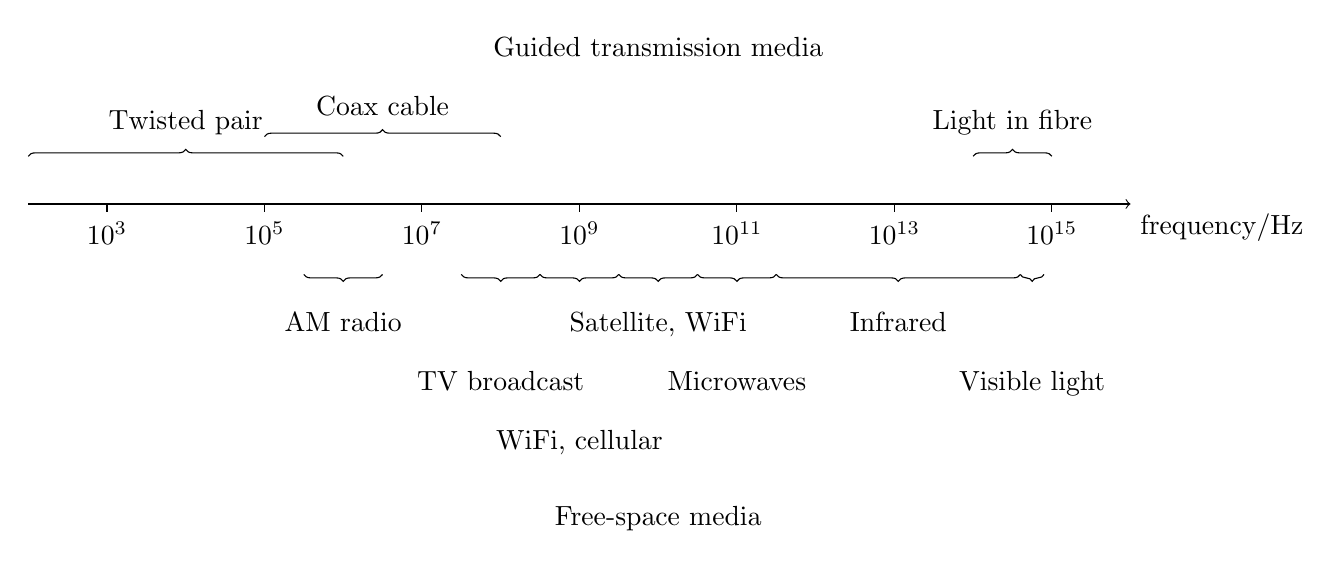
\begin{tikzpicture}
  \label{page:phy:media}


  \draw [->] (2,0) --  (16,0) node[below right] {frequency/Hz};

  \foreach \p in {3,5,...,15} {
    \draw (\p,0) -- (\p, -0.1) node [below] {$10^{\p}$};
  }


  \draw [decorate,decoration={brace, raise=3pt}] (2,0.5) to node[above=0.25] {Twisted pair} (6,0.5);  

  \draw [decorate,decoration={brace, raise=3pt}] (5,0.75) to node[above=0.25] {Coax cable} (8,0.75);  

  \draw [decorate,decoration={brace, raise=3pt}] (14,0.5) to node[above=0.25] {Light in fibre} (15,0.5);  

  \node at (10,2) {Guided transmission media};
  \node at (10,-4) {Free-space media};

  \draw [decorate,decoration={brace, mirror, raise=-3pt}] (5.5,-1) to node[below=0.25] {AM radio} (6.5,-1);  
  \draw [decorate,decoration={brace, mirror, raise=-3pt}] (7.5,-1) to node[below=1] {TV broadcast} (8.5,-1);  
  \draw [decorate,decoration={brace, mirror, raise=-3pt}] (8.5,-1) to node[below=1.75] {WiFi, cellular} (9.5,-1);  
  \draw [decorate,decoration={brace, mirror, raise=-3pt}] (9.5,-1) to node[below=0.25] {Satellite, WiFi} (10.5,-1);  
  \draw [decorate,decoration={brace, mirror, raise=-3pt}] (10.5,-1) to node[below=1] {Microwaves} (11.5,-1);  
  \draw [decorate,decoration={brace, mirror, raise=-3pt}] (11.5,-1) to node[below=0.25] {Infrared} (14.6,-1);  
  \draw [decorate,decoration={brace, mirror, raise=-3pt}] (14.6,-1) to node[below=1] {Visible light} (14.9,-1);  

  % https://en.wikipedia.org/wiki/Radio_spectrum
  
\end{tikzpicture}


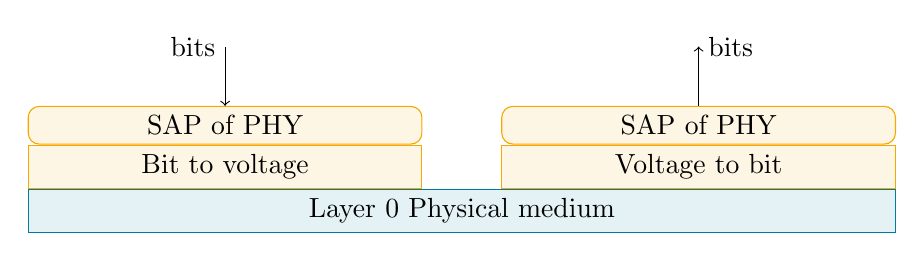
\begin{tikzpicture}
  \label{page:phy:service}

  \node [fill=hpiyellow!10, draw=hpiyellow,  rounded corners, minimum width=5cm] (sapl) {SAP of PHY};
  \node [fill=hpiyellow!10, draw=hpiyellow, below=0 of sapl, minimum width=5cm] (protl) {Bit to voltage};

  \node [fill=hpiyellow!10, draw=hpiyellow,  rounded corners, minimum width=5cm, right=of sapl] (sapr) {SAP of PHY};
  \node [fill=hpiyellow!10, draw=hpiyellow, below=0 of sapr, minimum width=5cm] (protr) { Voltage to bit};

  \node [fill=hpiblue!10, draw=hpiblue, below=0 of -(protl)(protr)] {Layer 0 Physical medium}; 

  \draw [<-] (sapl) -- ++ (0,1) node[left] {bits}; 
  \draw [->] (sapr) -- ++ (0,1) node[right] {bits}; 
  
\end{tikzpicture}

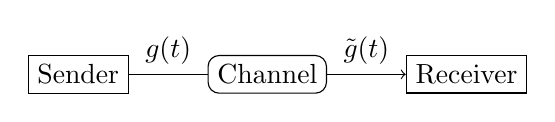
\begin{tikzpicture}
  \label{page:fig:channel}
  \node [draw] (sender) {Sender};
  \node [draw, rounded corners, right=of sender] (channel) {Channel};
  \node [draw, right=of channel] (rec) {Receiver};

  \draw [->] (sender) to node[above] {$g(t)$} (channel) to node[above] {$\tilde{g}(t)$} (rec); 
  
\end{tikzpicture}




\end{document}